\chapter{Flavor-Violating Interactions in Quantum Field Theory}
\label{fv_qft}

\section{Introduction}

If we are to discuss flavor violation, we must clarify what is meant by the {\it flavor} of a particle in the first place. Luckily, this does not involve licking any particles, but instead involves examining the fermion content of the Standard Model (SM). After electroweak symmetry breaking (EWSB), the SM fermions can be split into four sectors\footnote{Strictly speaking, these sectors are known as {\it super-selection sectors}, and restrict allowable quantum states to those whose kets transform identically under a gauge transformation.} according to their electromagnetic and color charges: there are the charged leptons, neutral leptons (or neutrinos), up-type quarks, and down-type quarks. Each of these sectors contains three fermions, any superposition of which constitutes a valid quantum state. Those superpositions which diagonalize the mass matrix of the fermions within a sector are given a   flavor label, so the flavors can be defined as the names given to the mass eigenstates of the fermions within a sector. When the fermions within each sector are sorted according to their mass, they are said to be assorted according to their {\it generation} (so the lightest fermions within each sector belong to the {\it first} generation of fermions and so on). 

This definition of flavor leaves some ambiguity as to the flavors of the neutrino sector, because (at least in the present form of the SM) the neutrinos are three-fold degenerate due to the lack of a neutrino mass matrix. As we will explore in more detail in Section \ref{sec:SM_FV}, this allows us to define the neutrino flavors to {\it align} with the charged lepton flavors. This is why we typically only speak of {\it three} lepton flavors ($e$, $\mu$, and $\tau$), but {\it six} quark flavors (the up-type $u$, $c$, and $t$, and the down-type $d$, $s$, and $b$). Contrary to the prediction of the SM, we know from astrophysical experiments that neutrinos do indeed have mass, as discussed in the Introduction. A more precise determination of the neutrino masses may ultimately lead to a naming convention of the neutrino mass eigenstates,\footnote{I propose the {\it iota}, {\it mote}, and {\it whit} neutrinos.} which would give a distinct set of neutrino flavors. Nevertheless, we would still be free to express the neutrino mass eigenstates in the charged lepton flavor basis, just as we can express the down-type quark mass eigenstates in the up-type quark flavor basis. The freedom to express the fermions of one sector in the flavor-basis of fermions in another sector is unique to the SM, since there is only one flavor-changing current (the $W$-boson interaction). 

Somewhat confusingly, {\it flavor violation} does not directly correspond to a process which changes particles of one flavor to particles of another flavor. Rather, the term flavor-violating is reserved for interactions that contribute to flavor-changing {\it neutral} currents. In other words, an interaction is said to be  flavor violating if it can lead to flavor transitions {\it within} one of the sectors of fermions described above. This can occur in one of two ways:
\begin{enumerate}
    \item A charged particle exists which permits transitions {\it between} sectors, and multiple exchanges of this charged particle can lead to transitions {\it within} a sector.
    \item A neutral particle exists which directly permits transitions from one flavor to another {\it within} a sector.
\end{enumerate}
The $W$-boson interaction is of type (1), and there are no known interactions of type (2). Nevertheless, interactions of type (2) are prevalent in models of new physics, and will be the primary focus of this dissertation.


This chapter is by no means exhaustive, but serves to explore some features and examples of flavor-violation in field theories that will be studied in subsequent chapters. In Section \ref{sec:SM_FV}, we will examine in detail how the flavor violation described above occurs in the quark sector of the SM but not the lepton sector. In Section \ref{sec:FV_scalars}, we will explore the symmetry properties of flavor-violating scalars and discuss some examples of flavor-violating scalars in models of new physics. In Section \ref{sec:ALP}, we will explore a special class of flavor-violating scalars: flavor-violating {\it axion-like particles}, which are of phenomenological interest. Finally,  in Section \ref{sec:U1_bosons}, we will discuss dark $U(1)$ gauge bosons, some of which exhibit lepton flavor violating couplings after spontaneous breaking of their gauge symmetry. 

\section{Flavor Violation in the SM}\label{sec:SM_FV}
While flavor violation is present in the quark sector of the SM, it is apparently absent in the lepton sector. To understand this disparity, we can examine the differences between these sectors by expanding the SM in unitarity gauge. As a reminder, the SM gauge group is $SU(3)_C \times SU(2)_L \times U(1)_Y$, and unitarity gauge is defined as the gauge for which the Higgs field $H$ (which has representation $(1, 2)_{1/2}$ under the SM gauge group) is parametrized by $H = e^{i\tau^a\xi_a}(0, \phi)$, where $\phi$ is a real scalar field, $\xi_a$ are its angular modes, and $\tau_a$ are the $SU(2)_L$ generators.

We begin with the quark sector. Prior to EWSB, the quark fields are defined as a flavor triplet of Weyl fermions ${\bf Q}$, ${\bf U}_{R}$, and ${\bf D}_{R}$ with charges $(3, 2)_{1/6}$, $(3, 1)_{1/3}$, and $(3, 1)_{-2/3}$ under the SM gauge group. Flavor-violation in the quark sector arises from a disparity between the quark-$W$ boson interactions and the quark-Higgs interactions. By expressing the quark $SU(2)_L$ doublet as ${\bf Q} = e^{i\tau^a\xi_a}({\bf U}_L, {\bf D}_L)$, we can extract the $W$-boson interaction from the kinetic term:
\begin{align}
    {\cal L}_{Q,{\rm kin.}} = \overline{\bf Q}[i\slashed{\partial}-g\tau^a \slashed{W}_a-\cdots]{\bf Q} &=\cdots - \frac{g}{\sqrt{2}}\overline{\bf U}_L \slashed{W}^+{\bf D}_L - \frac{g}{\sqrt{2}}\overline{\bf D}_L \slashed{W}^-{\bf U}_L+\cdots \nonumber\\
    &=\cdots - \frac{g}{\sqrt{2}}\overline{\bf U}{\slashed{W}}^+P_L{\bf D} + \cdots + {\rm H.c.}\label{eq:Q_W_int}
\end{align}
where we have only explicitly included the $SU(2)$ generators in the covariant derivative, and later singled out the $W$-boson interactions.\footnote{The insertion of the left-projection operator $P_L$ ensures that only the $W$-boson only interacts with the left-handed component of the quarks.} In addition, there are the Higgs Yukawa interaction terms:
\begin{align}
    {\cal L}_{Q,{\rm Yuk.}} &=  [\overline{\bf Q}H]{\bf Y}^u{\bf U}_R + [\overline{\bf Q}\tilde{H}]{\bf Y}^d{\bf D}_R + {\rm H.c.}\nonumber \\
    &= \phi[\overline{\bf U}_L{\bf Y}^u {\bf U}_R+\overline{\bf U}_R{\bf Y}^{\dagger u} {\bf U}_L] + \phi[\overline{\bf D}_L{\bf Y}^d {\bf D}_R+\overline{\bf D}_R{\bf Y}^{\dagger d} {\bf D}_L].
\end{align}
In this form, while the interaction in Eq.~\ref{eq:Q_W_int} is diagonal in flavor space (i.e. the interaction $\overline{\bf U}{\slashed{W}^+}P_L{\bf D} = \sum_i\overline{U}_i \slashed{W}^+P_LD_i$ only couples up- and down-type quarks of the same index $i$), the same cannot be said about the Yukawa term, due to the presence of the complex $3\times 3$ matrices (in flavor space) ${\bf Y}^u$ and ${\bf Y}^d$. In order for quark flavor to be preserved, it must be possible to simultaneously diagonalize the Higgs interactions and the $W$ interactions. We can try this explicitly, using singular value decomposition to write the Yukawa matrices as ${\bf Y}^q = {\bf V}_{qL}{\bf y}^q {\bf V}_{qR}^\dagger$, where ${\bf V}_{qL}$ and ${\bf V}_{qR}$ are unitary matrices and ${\bf y}^q$ is diagonal and Hermitian. Then, we are free to diagonalize the Yukawa terms via the field redefinition ${\bf q}_L = {\bf V}_{qL}^\dagger {\bf Q}_L$ and ${\bf q}_R = {\bf V}_{qR}^\dagger {\bf Q}_R$, and see what effect these transformations have on the $W$-boson interaction. While the Yukawa term 
\begin{align}
    {\cal L}_{Q,{\rm Yuk.}} 
    &= \phi[\overline{\bf u}_L{\bf y}^u {\bf u}_R+\overline{\bf u}_R{\bf y}^{u} {\bf u}_L] + \phi[\overline{\bf d}_L{\bf y}^d {\bf d}_R+\overline{\bf d}_R{\bf y}^{d} {\bf d}_L]\nonumber\\
    &= \phi\overline{\bf u}{\bf y}^u {\bf u} + \phi\overline{\bf d}{\bf y}^d {\bf d}
\end{align}
is now clearly diagonal, the $W$-boson interaction
\begin{align}
    {\cal L}_{Q,W} &= -\frac{g}{\sqrt{2}} \overline{\bf u}\slashed{W}^+P_L{\bf V}_{uL}^\dagger {\bf V}_{dL}{\bf d} + {\rm H.c.}
\end{align}
now contains a matrix ${\bf V}_{uL}^\dagger {\bf V}_{dL}$. This matrix is called the {\it CKM Matrix} (defined ${\bf V}_{\rm CKM} \equiv {\bf V}_{uL}^\dagger {\bf V}_{dL}$) due to the work of Cabibbo, Kobayashi, and Maskawa \cite{Cabibbo:1963yz,Kobayashi:1973fv}. Notably, this matrix is an arbitrary complex matrix, and is hence generally non-diagonal, so one can expect the $W$ boson interaction to induce mixing between the different flavors of quark. In particular, the magnitudes of the elements of the CKM matrix are given by \cite{ParticleDataGroup:2024cfk}
\begin{align}
    |{\bf V}_{\rm CKM}| \approx \begin{bmatrix} 0.974 & 0.225 & 0.004 \\ 
                                                0.225 & 0.973 & 0.042 \\
                                                0.009 & 0.041 & 0.999
                                \end{bmatrix}.
\end{align}
Interestingly, the matrix is {\it nearly} flavor-diagonal,\footnote{Given that $V_{\rm CKM}$ is {\it a priori} an arbitrary complex matrix, its closeness to unity is a mystery.} but there is a small degree of flavor-violation induced by the non-zero off diagonal components. Hence one has a choice: either the interaction with the Higgs preserves quark flavor, and the interaction with the $W$-boson is generically flavor-changing, or vice-versa. Given that the Higgs Yukawa interactions give rise to the fermion masses after EWSB and all of the standard formalism of QFT describes particles in terms of their mass eigenstates, it is convention to diagonalize these terms and leave the flavor-changing CKM matrix in the $W$-boson sector.


So why doesn't this happen in the lepton sector? Similar to before, the leptons are defined as a flavor triplet of Weyl fermions ${\bf L}$ and ${\bf E}_R$ with charges $(1, 2)_{-1/2}$ and $(1, 1)_{-1}$ respectively, and the doublet can be represented as ${\bf L} = e^{i\tau^a\xi_a}({\bf N}_L, {\bf E}_L)$ in unitarity gauge. The leptonic interaction with the $W$ can be found in the kinetic term of the leptonic $SU(2)$ doublet ${\bf L}$:
\begin{align}
{\cal L}_{L,{\rm kin}.} = \overline{\bf L}\left[i\slashed{\partial} - g\tau^a \slashed{W}_a - \cdots \right]{\bf L} &= \cdots -\frac{g}{\sqrt{2}}\overline{\bf N}_L\slashed{W}^+{\bf E}_L -\frac{g}{\sqrt{2}}\overline{\bf E}_L\slashed{W}^-{\bf N}_L + \cdots \nonumber \\
&= -\frac{g}{\sqrt{2}}\overline{\bf N}\slashed{W}^+P_L{\bf E} + {\rm H.c.}.
\end{align}
Whereas the lepton-Higgs Yukawa interaction is given by
\begin{align}
{\cal L}_{L,{\rm Yuk}.} &= [\overline{\bf L}H]{\bf Y}^\ell{\bf E}_R + {\rm H.c.}\nonumber \\
&= \phi [\overline{\bf E}_L{\bf Y}^\ell{\bf E}_R+\overline{\bf E}_R{\bf Y}^{\dagger e}{\bf E}_L]
\end{align}

Like before, the $W$ interaction is diagonal and the Higgs interaction is non-diagonal, but we can diagonalize ${\bf Y}^\ell$ using singular value decomposition ${\bf Y}^\ell = {\bf V}_{\ell L} {\bf y}^\ell{\bf V}_{\ell R}^\dagger$. Then, defining the charged lepton fields as ${\boldsymbol\ell}_{R,L} = {\bf V}_{\ell R,L}^\dagger{\bf E}_{R,L}$, the Yukawa interaction is given by
\begin{align}
    {\cal L}_{L,{\rm Yuk}} &= \phi\left[\overline{\boldsymbol \ell}_L{\bf y}^\ell {\boldsymbol \ell}_R + \overline{\boldsymbol \ell}_R{\bf y}^\ell {\boldsymbol \ell}_L\right]= \phi \overline{\boldsymbol \ell}{\bf y}^\ell{\boldsymbol\ell}
\end{align}

While this would seemingly introduce a non-diagonal coupling for the $W$-boson analogously to the quark case, the key difference is that we still have the freedom to rotate the neutrino flavors via the field redefinition ${\boldsymbol{\nu}}_L = {\bf V}_{\ell L}^\dagger {\bf N}_L$, due to the absence of a neutrino Yukawa matrix ${\bf Y}^\nu$.  Then, using the property ${\bf V}_{\ell L}^\dagger {\bf V}_{\ell L} = {\bf 1}$, we find 
\begin{align}
    {\cal L}_{L,W} &= -\frac{g}{\sqrt{2}}\overline{\boldsymbol \nu}{\slashed W}^+P_L{\boldsymbol \ell} + {\rm H.c.}
\end{align}
Hence, the $W$-boson interaction still preserves lepton flavor in the SM. By the same token, we can see that the lepton flavor symmetry is hanging on by a thread. In analogy with the quark sector, all it would take to dismantle this symmetry is the introduction of a SM singlet (under {\it all} the gauge groups) ${\bf N}_R$, which would act as a right-handed neutrino. This would require an additional set of rotation matrices ${\bf V}_{\nu L}$ and ${\bf V}_{\nu R}$ to diagonalize the Yukawa interaction,\footnote{More generally, the right-handed neutrino could have a Majorana term, and the total mass matrix (Majorana + Dirac) would have to be diagonalized, leading to flavor violation in both the Higgs {\it and} $W$-boson interactions.} which would in turn generate a CKM-like matrix for the lepton sector. Indeed, LFV has already been observed in the neutrino sector, as highlighted in the introduction. The CKM-like matrix is called the Pontecorvo-Maki-Nakagawa-Sakata, or PMNS, Matrix \cite{Pontecorvo:1967fh,Maki:1962mu}. Perhaps it is not surprising that one of the only pieces of evidence for physics beyond the SM (BSM) is an LFV signal.

\section{Flavor-Violating Scalars}\label{sec:FV_scalars}

Scalar fields are the simplest fields that one can study in relativistic quantum field theories. Scalar fields are realized in the SM through the Higgs field, which is a charged, complex scalar field before EWSB, and a real scalar field after EWSB. Scalar fields are also ubiquitous in BSM theories of physics. Here we will review some of the properties of scalars with flavor-violating interactions, as well as some examples of BSM scalars. 


\subsection{Symmetry Properties of FV Scalar Interactions}\label{sec:FV_scalar_CPT}


The most generic interaction between charged\footnote{If they were uncharged, one could also have the terms $\phi\bar{\psi}_i^c \Gamma_{ij}\psi_j$. Alternatively, if $\varphi$ is complex and charged under the same symmetry as the $\psi_i$, then this term can occur.} spin-1/2 Dirac fermions $\psi_i$ and a real scalar $\varphi$ is given by
\begin{align}
    {\cal L} &= \sum_{i,j}\bar{\psi}_i(g_{ij}^{S} + ig_{ij}^{PS}\gamma^5)\psi_j \varphi \label{eq:phi_int}
\end{align}
where, $g_{ij}^S$ and $g_{ij}^{PS}$ are complex numbers that describe the strength of the interaction. In order to ensure that the Lagrangian is real, it is required that $g_{ij}^S = g_{ji}^{S*}$ and $g_{ji}^{PS} = g_{ji}^{PS*}$. In particular, this means that the on-diagonal (flavor-preserving) couplings must be real. When only the left (right) coupling in Eq.~\ref{eq:phi_int} is present, the $\phi$ is referred to as a (pseudo)scalar. This can be understood by examining the parity transformation of the interaction. Parity acts on the interaction term as
\begin{align}
    {\rm P}^{-1}{\cal L}{\rm P} &= \sum_{i,j}{\rm P}^{-1}\bar{\psi}_i(g_{ij}^{S} + ig_{ij}^{PS}\gamma^5)\psi_j {\rm P}{\rm P}^{-1}\varphi{\rm P} \nonumber\\
    &= \sum_{i,j}\bar{\psi}_i(g_{ij}^{S} - ig_{ij}^{PS}\gamma^5)\psi_j {\rm P}^{-1}\varphi{\rm P}.
\end{align}
Note that for a general coupling, one cannot consistently assign a parity charge for $\varphi$ that leaves the interaction term invariant under a parity transformation. However, if $g_{ij}^{PS} = 0$, then one can choose ${\rm P}^{-1}\varphi {\rm P} = +\varphi$, and if $g_{ij}^{S} = 0$, then one can choose ${\rm P}^{-1}\varphi {\rm P} = -\varphi$. Hence, if only the left coupling is present, $\varphi$ transforms as a scalar under parity, and if only the right-coupling is present, $\varphi$ transforms as a pseudoscalar under parity. If we instead apply charge-conjugation, we have
\begin{align}
    {\rm C}^{-1}{\cal L}{\rm C} &= \sum_{i,j}{\rm C}^{-1}\bar{\psi}_i(g_{ij}^{S} + ig_{ij}^{PS}\gamma^5)\psi_j {\rm C}{\rm C}^{-1}\varphi{\rm C} \nonumber\\
    &= \sum_{i,j}\bar{\psi}_j(g_{ij}^{S} + ig_{ij}^{PS}\gamma^5)\psi_i {\rm C}^{-1}\varphi{\rm C} \nonumber\\
    &= \sum_{i,j}\bar{\psi}_i(g_{ij}^{S*} + ig_{ij}^{PS*}\gamma^5)\psi_j \varphi.
\end{align}
Here, we cannot assign a C-charge to $\varphi$ as it is a real scalar. We see that charge-conjugation-symmetry is obeyed precisely when the couplings are strictly real. Combining both yields the CP transformation
\begin{align}
    {\rm CP}^{-1}{\cal L}{\rm CP} 
    &= \sum_{i,j}\bar{\psi}_i(g_{ij}^{S*} - ig_{ij}^{PS*}\gamma^5)\psi_j {\rm CP}^{-1}\varphi{\rm CP}.
\end{align}
It follows that for flavor-preserving ($j = i$) couplings, $\varphi$ can be designated CP-even if $g_{ij}^{S*} = g_{ij}^S$ and $g_{ij}^{PS*} = -g_{ij}^{PS}$, and CP-odd if $g_{ij}^{S*} = -g_{ij}^{S}$ and $g_{ij}^{PS*} = g_{ij}^{PS}$. More generally, if there is still freedom to absorb phases into the fermion fields, then the term can be made CP-conserving as long as ${\rm arg}(g_{ij}^{S}) = {\rm arg}(ig_{ij}^{PS})$.

It is sometimes convenient to parametrize the interaction in terms of angles and phases. In particular, we define $g_{ij} = \sqrt{|g_{ij}^S|^2 + |g_{ij}^{PS}|^2}$, $\theta_{ij} = \arctan(|g_{ij}^{PS}/g_{ij}^S|)$, and $\phi_{ij}^{(P)S} ={\rm arg}(g_{ij}^{(P)S})$. We also define $\delta_{ij} = \phi_{ij}^{PS} - \phi_{ij}^S$ so that we can highlight the difference in phases between the two terms. Then the interaction is of the form
\begin{align}
    {\cal L} &= \sum_{ij}g_{ij}e^{i\phi_{ij}^S}\bar{\psi}_i(\cos{\theta_{ij}} + ie^{i\delta_{ij}}\sin{\theta_{ij}}\gamma^5)\psi_j \varphi.
\end{align}
Without loss of generality, we can take $\theta_{ij} \in [0, \pi/2]$. Then, the reality condition becomes $g_{ij} = g_{ji}$, $\theta_{ij} = \theta_{ji}$, $\phi_{ij}^{(P)S} + \phi_{ji}^{(P)S} = 0$, and $\delta_{ij} + \delta_{ji} = 0$. The on-diagonal phases satisfy $\phi_{ij}^{(P)S} = \delta_{ij} = 0$, as expected. Such a parametrization is useful when calculating Feynman diagrams,  where one can use trigonometric identities to simplify expressions. In this notation, we see that $\theta_{ij}$ directly controls the degree of parity-violation (PV), $\phi_{ij}^S$ and $\phi_{ij}^{PS}$ controls the degree of C-violation, and $\delta_{ij} = \phi_{ij}^{PS} - \phi_{ij}^{S}$ controls the degree of CP-violation (CPV). 

The situation for a complex scalar is (ironically) simpler, in the sense that the couplings, angles and phases are now free to be chosen independently, as there is no reality condition to satisfy. The trade-off is that an interaction with an outgoing $\varphi$ is the complex-conjugate of an interaction with an ingoing $\varphi$. One phenomenologically interesting case is when the angles and phases are chosen such that the complex scalar interacts chirally with the fermions; that is, $\theta_{ij} = \pi/4$ and $\delta_{ij} = \pm \pi/2$. This situation is often well-motivated due to the chiral nature of the SM fields. Indeed, this is the case for the Higgs interaction with fermions before EWSB occurs. 

It should be noted that the complex scalar can be written as two real scalars $\varphi = \varphi_r + i\varphi_i$. Written in this form, the reality condition implies that the $\varphi_r$ plays the role of a scalar and the $\varphi_i$ plays the role of a pseudoscalar, at least for the on-diagonal couplings. However as we have seen, even these real fields can have non-diagonal interactions for which there is no consistent choice of parity.


\subsection{Two-Higgs-Doublet Model}\label{sec:2HDM}
What if there were a second Higgs? This is the question that the two-Higgs doublet model (2HDM) aims to answer. The question is far from arbitrary, as a second Higgs doublet is required in supersymmetric extensions of the SM \cite{Haber:1984rc,Csaki:1996ks}, appears in the spectrum of many grand-unified theories {\color{red} \cite{}}, and also can appear in models that provide a neutrino mass mechanism \cite{Ma:2000cc,Gabriel:2006ns,Wang:2006jy} or a candidate for dark matter \cite{Ma:2006fn,Ma:2006km,Aoki:2008av}. Here we will divorce the second Higgs doublet from any particular new model of physics, and instead consider the broad ramifications one can expect from its inclusion. For a review of 2HDMs, we refer to Refs.~\cite{Aoki:2009ha,Branco:2011iw,Wang:2022yhm}.

We call the two Higgs doublets $\Phi_1$ and $\Phi_2$. Unless one imposes additional symmetries, each of them has the same interactions with the fermions as the SM Higgs field. These are
 \begin{align}
    {\cal L}_{\rm Yuk.} &= \left[\overline{\bf L}\Phi_1\right]{\bf Y}_1^\ell {\bf E}_R + \left[\overline{\bf Q}\Phi_1\right]{\bf Y}_1^u {\bf U}_R + \left[\overline{\bf Q}\tilde{\Phi}_1\right]{\bf Y}_1^d {\bf D}_R \nonumber \\
    &+ \left[\overline{\bf L}\Phi_2\right]{\bf Y}_2^\ell {\bf E}_R + \left[\overline{\bf Q}\Phi_2\right]{\bf Y}_2^u {\bf U}_R + \left[\overline{\bf Q}\tilde{\Phi}_2\right]{\bf Y}_2^d {\bf D}_R + {\rm H.c.}
 \end{align} 
Referring to Section \ref{sec:SM_FV}, we can already see how such a model will lead to flavor violation in the lepton sector and additional flavor violation in the quark sector: After spontaneous breaking of the electroweak symmetry,  the mass matrices will be obtained from singular value decomposition of the matrix ${\bf M}^f = v_1{\bf Y}_1^f + v_2{\bf Y}_2^f$, where $v_1$ and $v_2$ are the vacuum expectation values (VEVs) of $\Phi_1$ and $\Phi_2$. Unlike in the SM, diagonalization of ${\bf M}^f$ will generically not diagonalize either of the Higgs interactions, so one can expect each scalar in the theory to have flavor-violating couplings. Flavor-violating interactions with the SM Higgs have yet to be observed, which places limits on the strength of the Yukawa couplings and size of the second Higgs VEV. It should also be noted that an additional Higgs doublet introduces not one, but {\it five} new real scalar fields after EWSB.\footnote{This is because each Higgs doublet has two complex (four real) degrees of freedom, and only three degrees of freedom are ``eaten'' by the gauge fields corresponding to the broken generators of the electroweak symmetry.} After diagonalization of the fermion mass matrices, each of these will have flavor-violating couplings unless a symmetry is explicitly imposed to prevent them. In Type I Type II, lepton-specific (or Type X), and flipped (or Type Y) 2HDMs, a discrete ${\Bbb Z}_2$ symmetry is imposed that restricts each Higgs doublet to interact with different fermion sectors, which has the effect of forbidding tree-level flavor-changing neutral currents \cite{Glashow:1976nt,Paschos:1976ay,Aoki:2009ha,Branco:2011iw,Wang:2022yhm}. However, the most general incarnation of the 2HDM has flavor-violating scalars whose mass and couplings are constrained by experiments \cite{Harnik:2012pb,Primulando:2019ydt}.


\subsection{Froggatt-Nielsen Models}\label{sec:FN}
One of the biggest outstanding problems in particle physics is the fermion hierarchy problem: why is there such a large separation of scales between the observed masses of each generation of fermions? Ignoring the neutrinos (whose internal hierarchy is unknown and which may very well get their low masses through a different mechanism than the other fermions), the other sectors have hierarchies of $m_\tau/m_e \approx 3.5\times 10^3$, $m_b/m_d \approx 900$, and $m_t/m_u \approx 8\times 10^4$ between their first and third generations. While such hierarchies can be obtained by simply asserting that the Higgs Yukawa matrices are hierarchical, this explanation is unsatisfactory for most particle physicists.

Froggatt-Nielsen models attempt to solve this problem by introducing a global horizontal symmetry group $U(1)_H$ along with a generation-dependent charge structure for the SM fermions \cite{Froggatt:1978nt}. Generically, the left- and right-handed fermion fields of each generation have different $U(1)_H$ charges, so $Q_H[F_{i}] = q^{F}_i$ and $Q_H[F_{Ri}]\equiv q^{F_R}_i$. This has the effect of forbidding the usual SM Yukawa terms
\begin{align}
    {\cal L}_{\rm Yuk} = \sum_{i,j}\left[Y_{ij}^\ell\bar{L}_{i} H E_{Rj} +Y_{ij}^u\bar{Q}_{i} H U_{Rj} +Y_{ij}^d\bar{Q}_{i} \tilde{H} D_{Rj} \right] + {\rm H.c.}
\end{align}
as these terms have $U(1)_{H}$ charge $q_i^{F_R} - q_j^{F} \neq 0$. These terms are restored by introduction of a complex scalar field $\Phi$, the flavon, with $U(1)_H$ charge $1$. Then, the charge $q_i^{F_R} - q_j^{F}$ can be canceled by powers of the flavon, $\Phi^{q_i^{F} - q_j^{F_R}}$. The lowest-order effective field theory (EFT) term is then
\begin{align}
    {\cal L}_{\rm FN} = \sum_{i,j}\left[X_{ij}^\ell\left(\frac{\Phi}{M}\right)^{n_{ij}^\ell}\bar{L}_{i} H E_{Rj} +X_{ij}^u\left(\frac{\Phi}{M}\right)^{n_{ij}^u}\bar{Q}_{i} H U_{Rj} +X_{ij}^d\left(\frac{\Phi}{M}\right)^{n_{ij}^d}\bar{Q}_{i} \tilde{H} D_{Rj} \right] + {\rm H.c.}
\end{align}
where $n_{ij}^f \equiv q_i^{F} - q_j^{F_R}$ and $X_{ij}^f$ are ${\cal O}(1)$ couplings. If the flavon acquires a VEV $v_\Phi \ll M$, this will naturally generate a hierarchy in the Yukawa couplings $Y_{ij}^f = X_{ij}^f(v_\Phi/M)^{n_{ij}^f} \sim X_{ij}^f\epsilon^{n_{ij}^f}$. The hierarchy of the fermion masses in the SM can be recovered by choosing appropriate values for $q_i^{F}$ and $q_i^{F_R}$. To get a sense of the charges required to reproduce the SM fermion mass spectrum, we refer to Ref.~\cite{Cornella:2024jaw}, which scans over valid Froggatt-Nielsen solutions to the fermion hierarchy problem with $|q_i^{F_R}|, |q_i^F| < 7$ (or $|q_i^{F_R}|, |q_i^F| < 9$ with the inclusion of three Dirac right-handed neutrinos).

In addition to the effective coupling between the flavon and the SM, the flavon has a potential, given by
\begin{align}
    V(\Phi) = \mu_\Phi^2 |{\Phi}|^2 + \frac{1}{2}\lambda_\Phi|\Phi|^4.\label{eq:FN_potential}
\end{align}
The global $U(1)_H$ symmetry is spontaneously broken when the flavon acquires a VEV $v_\Phi \neq 0$. This form of the potential motivates a decomposition of the flavon $\Phi$ in terms of its radial and angular components, $\Phi = (v_\Phi + \rho) e^{ia/v_\Phi} \sim v_\Phi + \rho + ia$. The leading order interaction of these fields with the SM fermion fields (after EWSB but {\it before} diagonalization of the mass matrices) is given by
\begin{align}
    {\cal L}_{\rm FN,  int.} &= \sum_{i,j}v_H Y_{ij}^f n_{ij}^f\frac{\rho + ia}{v_\Phi}\bar{F}_{Li} F_{Rj}.
\end{align}
Notably, the presence of $n_{ij}^f$ prevents simultaneous diagonalization of this interaction term with the Yukawa matrices $Y_{ij}^f$. Hence, we see that the Froggatt-Nielsen scalars generically appear with flavor-violating interactions. The degree to which these interactions are constrained by existing searches for flavor-violation is explored in Ref.~\cite{Cornella:2024jaw}. 

While the $\rho$ attains its mass from the potential (\ref{eq:FN_potential}) after $U(1)_H$ symmetry-breaking, the $a$ is a Goldstone boson of the $U(1)_H$ symmetry. However, the chiral nature of the $U(1)_H$ charges results in a chiral anomaly, so the $U(1)_H$ is approximate and the $a$ acquires a small mass. This property of the $a$ makes it an example of an {\it axion-like particle}, which are the subject of Section {\ref{sec:ALP}}. We will briefly return to the $a$, which is sometimes called the {\it axiflavon} \cite{Calibbi:2016hwq} or {\it flaxion} \cite{Ema:2016ops}, in Section {\ref{sec:FN_ALP}.

\section{Axion-Like Particles}\label{sec:ALP}
An axion-like particle (ALP) is a pseudo\footnote{{\it Pseudo} here refers to the fact that it is not a {\it true} Nambu-Goldstone boson, as it has a small mass by virtue of explicit symmetry breaking.}-Nambu-Goldstone boson (pNGB) that results from the spontaneous breaking of an approximate global symmetry. They are ubiquitous in extensions beyond the SM, as global symmetries are often imposed directly (as we have seen with Froggatt-Nielsen models), or arise accidentally from imposing gauge symmetries (as is the case with the lepton family, lepton number, and baryon number symmetries in the SM). For a review of ALPs in various contexts, see Refs.~\cite{Ringwald:2014vqa,Choi:2020rgn}.


The namesake of the ALP is a hypothetical particle called the axion, which was devised by Peccei and Quinn in the 1960s as a possible solution to the Strong CP problem \cite{Peccei:1977hh,Peccei:1977ur}. In short, the Strong CP problem is the observation that the CP-odd gluon-gluon interaction
\begin{align}
    {\cal L}_{\theta} &= \frac{\theta}{32\pi^2}{\rm Tr}\{G^{\mu\nu}\tilde{G}_{\mu\nu}\}\label{eq:theta_term}
\end{align}
is apparently absent from the SM, despite respecting all of the SM symmetries. Measurements of the neutron electric dipole moment indicate that $|\theta| < 10^{-13}$, whereas naturalness would predict $\theta = {\cal O}(1)$,\footnote{The problem is subtly worse. Since CP-violation exists in the CKM-matrix of the SM, (\ref{eq:theta_term}) receives loop-level corrections. To reproduce our observations, the {\it bare} $\theta$ must not be zero, but instead must conspire to exactly cancel out with quantum corrections from the quark sector at our energy scale. This is a fine-tuned scenario and hence an unsatisfactory solution for many physicists.} so physicists expect that there must be some mechanism at play to prevent this interaction. The axion is the pNGB of an anomalous $U(1)$ symmetry, whose VEV aligns with $\theta$ to dynamically force the term (\ref{eq:theta_term}) to zero. While the original axion model proposed by Peccei and Quinn has been ruled out, generalizations such as the DFSZ axion \cite{Dine:1981rt,Zhitnitsky:1980tq} and KSVZ axion \cite{Kim:1979if,Shifman:1979if}  still have a large parameter space untouched by modern experiments, and double as a promising candidate for dark matter \cite{Adams:2022pbo}. 

While the ALP is named after a particle that has yet to be observed, we need not look beyond the SM to find an example: the pions. In particular, the QCD Lagrangian for the two lightest quarks ($u$ and $d$) exhibits a global $SU(2)_L\times SU(2)_R$ chiral flavor symmetry in the limit of vanishing quark masses. This symmetry is explicitly broken by the quark Yukawa couplings and, to a much lesser extent, the electroweak interactions. Since the quark Yukawa couplings are small relative to the QCD confinement scale, this can be understood as an {\it approximate} global symmetry. At low temperatures, the QCD vacuum develops a chiral condensate that spontaneously breaks the chiral symmetry down to an $SU(2)_V$ isospin flavor symmetry, giving rise to three pseudo-Goldstone bosons. These are the pions $\pi^\pm$ and $\pi^0$, which acquire a small mass due to the explicit symmetry breaking, in accordance with Goldstone's theorem.\footnote{This same analysis can be extended to include the strange quark, so that a global $SU(3)_L \times SU(3)_R$ chiral flavor symmetry breaks to an $SU(3)_V$ isospin symmetry. In this case, there are eight Goldstone modes, associated with the eight mesons in Gell-Mann's ``eightfold way'' \cite{Gell-Mann:1961omu}. The remaining mesons, the eta ($\eta$) and the kaons ($K^\pm, K^0$), are heavier than the pions, because the strange quark breaks the approximate chiral symmetry much more than the up or down quarks ($m_s/(m_u + m_d) \approx 14$).} This introduces the possibility that ALPs can arise as pions from composite dark sectors. We will explore an example of this possibility in Section \ref{sec:composite_ALP}. 

Perhaps the most exciting feature of ALPs for a phenomenologist is that they are, by definition, much lighter than the energy-scale of the new physics from which they come. Coupled with the fact that generic ALP interactions mix both quark and lepton flavor, ALPs provide a tantalizing target for physics experiments. We will explore limits on ALPs from existing searches for LFV in Chapter~\ref{lfv}, and for a broader set of existing and upcoming collider experiments in Chapter~\ref{alp_collider}.


\subsection{ALP Effective Field Theory}\label{sec:ALP_EFT}
Here, we provide a brief overview of the low-energy EFT of the ALP. More detailed analyses of its structure and renormalization properties can be found in Refs. \cite{Georgi:1986df,Bauer:2017ris,Bauer:2020jbp,Bauer:2021mvw}. From their definition as pNGBs of some approximate global symmetry, all that is important for the EFT is that the ALP interactions obey a continuous shift symmetry $a \rightarrow a + {\rm const.}$ (characteristic of Nambu-Goldstone bosons) which is explicitly broken either by a term in the Lagrangian or by anomalous quantum effects. The symmetry can be imposed directly with terms of the form $\partial_\mu a\, {\cal O}$ and $e^{ia/f}{\cal O}$, where ${\cal O}$ is any SM gauge-invariant operator. However, the latter term subtly breaks the symmetry due to a chiral anomaly, so it is preferable to rotate the SM fields in such a way that remove these operators in favor of equivalent operators which demonstrate the symmetry-breaking more explicitly. In particular, performing the rotation not only modifies the coefficients of the $\partial_\mu a\,{\cal O}$ terms, but also introduces linear couplings to the gauge fields $a{\tilde F}F$. While these terms are sufficient to break the ALP's shift symmetry into a discrete symmetry, the shift symmetry may be broken explicitly by other means; this can be accounted for phenomenologically by allowing the ALP to have a mass $m_a$ (along with higher-order potential terms). All told, we have the low-energy effective Lagrangian \cite{Georgi:1986df,Bauer:2021mvw}
\begin{align}
    {\cal L}_{\rm ALP} &= \frac{1}{2}(\partial_\mu a)^2 - \frac{1}{2}m_a^2 a^2 - \frac{1}{\Lambda}\partial_\mu a\sum_{f,i,j}\bar{f}_i\gamma^\mu\left[V_{ij}^f - A_{ij}^f\gamma_5\right]f_j+ e^2 C_{\gamma\gamma}\frac{a}{\Lambda}F_{\mu\nu}\tilde{F}^{\mu\nu} + \cdots \nonumber\\
    &\ \ \ + \frac{1}{4}\lambda_a \frac{m_a^2}{\Lambda^2}a^4+ C_{ah}\frac{(\partial_\mu a)^2}{\Lambda^2}vh + C_{ah}'\frac{m_a^2 a^2}{\Lambda^2}vh + \cdots \label{eq:ALP_EFT}
\end{align}
where the dots on the first line include other ${\cal O}(\Lambda^{-1})$ interactions with gauge fields, and the dots on the second line include ${\cal O}(\Lambda^{-2})$ terms.\footnote{While these operators are not six-dimensional, the Higgs interactions are derived from six-dimensional operators prior to EWSB, and the quartic term in the ALP potential is anticipated to be suppressed by $(m_a/\Lambda)^2$ due to the approximate symmetry.} The Higgs couplings on the second line warrant extra discussion. The first obeys the shift symmetry and is thus generically allowed in the ALP effective theory. The second is explicitly symmetry violating, but can occur in some UV-completions for which the source of explicit symmetry breaking is an interaction with the Higgs (such as the model studied in Section~\ref{sec:composite_ALP}). Phenomenological constraints on these couplings in the context of LFV ALPs are presented in Chapter {\ref{alp_collider}}.

While the derivative coupling of the ALP to fermions emphasizes the shift symmetry, it is possible to integrate the fermion interaction term by parts and use the equations of motion to obtain a standard scalar interaction for the ALP,
\begin{align}
    \frac{1}{\Lambda}\partial_\mu a \sum_{f,i,j}\bar{f}_i\gamma^\mu\left[V_{ij}^f - A_{ij}^f \gamma_5\right]f_j \longrightarrow  -ia \sum_{f,i,j}\bar{f}_i\gamma^\mu\left[\frac{m_i - m_j}{\Lambda}V_{ij}^f + \frac{m_i + m_j}{\Lambda}A_{ij}^f \gamma_5\right]f_j.\label{eq:ALP_rewrite}
\end{align}
Written in this form, we see a hallmark feature of ALPs: they couple to fermions with a strength proportional to the mass of the fermions. This entails that (as long as the couplings $A_{ij}$ and $V_{ij}$ themselves are not hierarchical) ALPs will couple primarily to the third generation of fermions.

However, one cannot rewrite the fermion interaction as in Eq.~\ref{eq:ALP_rewrite} without inducing a modification to the gauge boson couplings, due to the chiral anomaly. For example, when the Lagrangian is rewritten in this form, the photon coupling becomes
\begin{align}
    \tilde{C}_{\gamma\gamma} &= C_{\gamma\gamma} + \sum_{f\in \{\ell, u, d\}}\sum_{i=1}^{3}\frac{N_c^fQ_f^2}{8\pi^2}A_{ii}^f, \label{eq:Cgg_eff}
\end{align}
and there are analogous formulae for the other gauge boson couplings \cite{Bauer:2021mvw}. An effective photon coupling is often cited as the full one-loop contribution to the coupling, given by
\begin{align}
    C_{\gamma\gamma}^{\rm eff.} &= C_{\gamma\gamma} + \sum_{f\in \{\ell, u, d\}}\sum_{i=1}^{3}\frac{N_c^fQ_f^2}{8\pi^2}A_{ii}^f B_1(4m_{f_i}^2 / m_a^2)
\end{align}
where
\begin{align}
    && B_1(\tau) = 1 - \tau f(\tau)^2, && f(\tau) = \begin{cases}\arcsin\frac{1}{\sqrt{\tau}}&\tau\geq1,\\\tfrac{\pi}{2}+\tfrac{i}{2}\log\frac{1+\sqrt{1-\tau}}{1-\sqrt{1-\tau}} & \tau < 1.\end{cases} && 
    \label{eq:B1}
\end{align}
However, we note that this formula is only strictly valid when the momenta are on shell, i.e. for the decay process $a\rightarrow \gamma\gamma$.  When the $a\gamma\gamma$ vertex appears inside a diagram, one must compute the full two-loop contribution to the diagram. Nevertheless, Eq.~\ref{eq:Cgg_eff} captures a useful qualitative feature of the vertex which survives the general off-shell treatment: light fermions contribute $N_c^f Q_f^2/8\pi^2 A_{ii}^f$ to the photon vertex whereas heavy fermions decouple. For a more rigorous two-loop treatment of $C_{\gamma\gamma}^{\rm eff.}$, we refer to Refs.~\cite{Buen-Abad:2021fwq,Neubert:2024jal}.

\subsection{ALP as a (Pseudo-)Scalar}\label{sec:ALP_as_pseudoscalar}
As seen in the previous section, ALPs can be treated as scalars by integrating by parts and using the equations of motion, at the expense of modifying the ALP-gauge boson coupling. Let us consider the interaction between an ALP $a$ and a set of fermions $\psi_i$:
\begin{align}
    {\cal L} &= \sum_{ij}\frac{\partial_\mu a}{\Lambda}\bar{\psi}_i\gamma^\mu(g^V_{ij} + g^A_{ij}\gamma_5)\psi_j.
\end{align}
To ensure the Lagrangian is real, we have $g_{ij}^{V}=g_{ji}^{V*}$, and $g_{ij}^{A} = g_{ji}^{A*}$.

After integrating by parts and applying the equations of motion, 
\begin{align}
    {\cal L} &= \sum_{ij}a\bar{\psi}_i\left[-i\frac{m_i - m_j}{\Lambda}g^V_{ij} -i\frac{m_i + m_j}{\Lambda}g^A_{ij}\gamma_5\right]\psi_j.
\end{align}
This can be matched directly onto the real scalar interaction term Eq.~\ref{eq:phi_int}, so that
\begin{align}
    g_{ij}^S = -i\frac{m_i-m_j}{\Lambda}g_{ij}^V, & &
    g_{ij}^{PS} = -\frac{m_i+m_j}{\Lambda}g_{ij}^A.
\end{align}
In particular, $g_{ij}^S = g_{ji}^{S*}$ and $g_{ij}^{PS} = g_{ji}^{PS*}$, as expected. This means that in principle, amplitudes calculated involving fermions and scalars can be easily recast to involve ALPs instead, or vice-versa. 

As before, we can define a magnitude $C_{ij} = \sqrt{|g_{ij}^A|^2 + |g_{ij}^V|^2}$,  angles $\Theta_{ij} = \arctan(|g_{ij}^{V}/g_{ij}^A|)$, and phases $\Phi_{ij}^{A,V} ={\rm arg}(g_{ij}^{A,V})$, with $\Delta_{ij} = \Phi_{ij}^A - \Phi_{ij}^V$. The resulting interaction Lagrangian is
\begin{align}
    {\cal L} &= \sum_{ij}\frac{\partial_\mu a}{\Lambda}C_{ij}e^{i\Phi_{ij}^V}\bar{\psi}_i\gamma^\mu(e^{i\Delta_{ij}}\sin{\Theta_{ij}} +\cos{\Theta_{ij}}\gamma_5)\psi_j.
\end{align}
It is then possible to directly recast the ALP parameters to the scalar parameters and vice-versa. For the magnitude and angles, we have
\begin{align}
    \frac{C_{ij}}{\Lambda} &= \frac{g_{ij}}{|m_i^2 - m_j^2|}\sqrt{m_i^2+m_j^2+2m_im_j\cos{2\theta_{ij}}} & \tan{\Theta_{ij}} &= \frac{m_i+m_j}{\left|m_i-m_j\right|}\cot{\theta_{ij}}\label{eq:scalar_to_ALP}
    \\
    g_{ij} &= \frac{C_{ij}}{\Lambda}\sqrt{m_i^2+m_j^2+2m_im_j\cos{2\Theta_{ij}}} & \tan{\theta_{ij}} &= \frac{m_i+m_j}{\left|m_i-m_j\right|}\cot{\Theta_{ij}}. \label{eq:ALP_to_scalar}
\end{align}
The phases require careful thought due to the sign of the $m_j - m_i$ term. In particular, if $\theta_{ij}$ is taken to be positive, then we must have $i{\rm sgn}(m_j - m_i)e^{i\Phi_{ij}^A} = e^{i\phi_{ij}^S}$ and $ie^{i\Phi_{ij}^V} = ie^{i\phi_{ij}^{PS}}$, which can be easily solved for the resulting phases. This can be avoided if $\theta_{ij}$ is allowed to run negative.

The term in the square-root invites the definition of a mass parameter 
\begin{align}
    m_{ij}(\gamma) = \sqrt{m_i^2 + m_j^2 + 2m_i m_j \cos{2\gamma}}
\end{align}
which often appears in Feynman amplitudes. When transferring from scalar notation to ALP notation, we can then use 
\begin{align}
    m_{ij}(\theta_{ij})m_{ij}(\Theta_{ij}) = |m_i^2 - m_j^2|.\label{eq:mass_rel}
\end{align}
Curiously, these equations appear to represent a geometric relationship between the parameters of the two equivalent EFT terms. In particular, the first and second column of Eqs.~(\ref{eq:scalar_to_ALP})-(\ref{eq:ALP_to_scalar}) look similar to the Law of Cosines and Law of Tangents, respectively. This relationship is represented graphically with the trapezoid in Fig.~\ref{fig:trapezoid}. We then recognize Eq.~\ref{eq:mass_rel} as the equation for the relationship between an isosceles trapezoid's diagonal and its side-lengths.

\begin{figure}
    \centering
    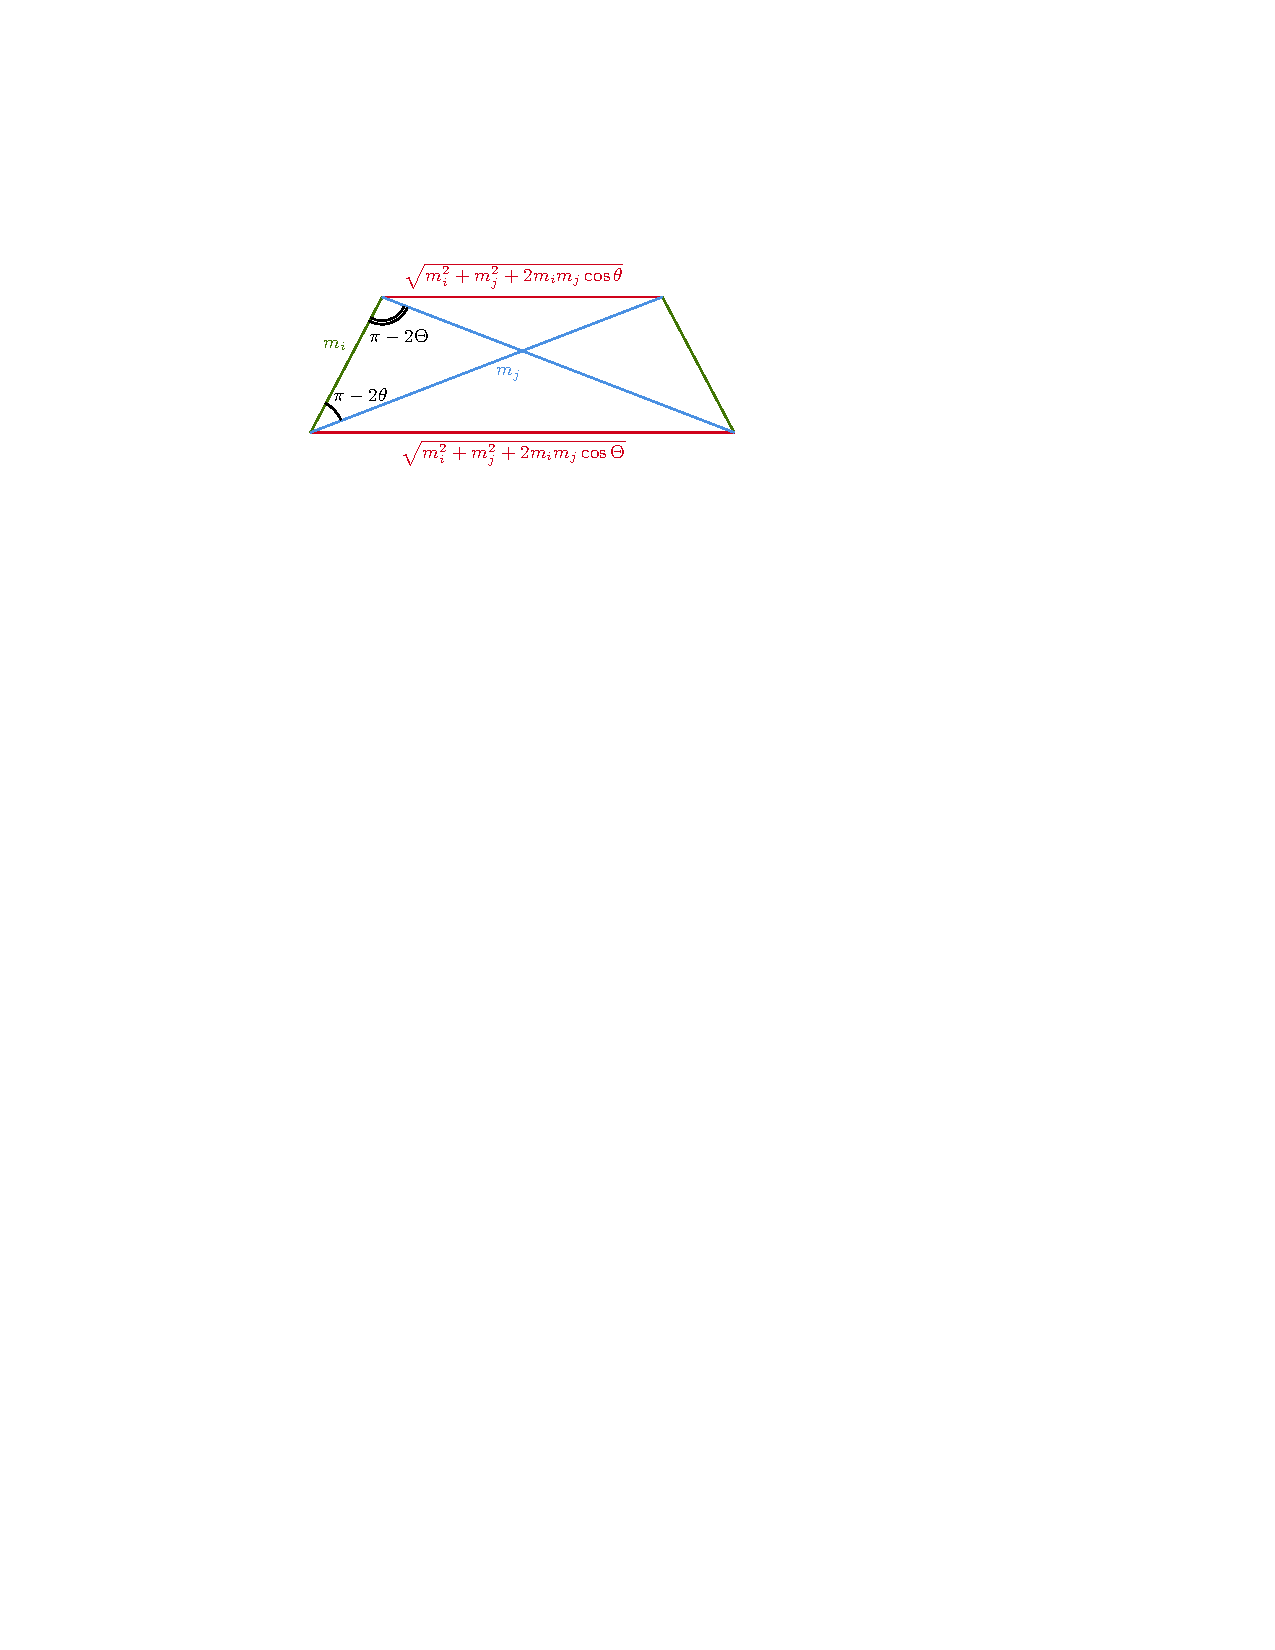
\includegraphics[width=0.5\linewidth]{figures/chapter2/trapezoid.pdf}
    \caption[A trapezoid which encodes the relationship between equivalent effective field theory terms.]{A trapezoid which encodes the relationship between the equivalent EFT terms. The indices on the angles are suppressed.} 
    \label{fig:trapezoid}
\end{figure}

It's unclear whether this geometric relationship is superficial or if there is a deeper interpretation. In the special case that the scalar couplings are pure real, one can always write the current in the interaction as $g \bar{\psi}_ie^{i\gamma_5 \theta_{ij}}\psi_j$ and define $\psi_{i}' = e^{i\gamma_5 \theta_{ij}/2}\psi_i$. This field redefinition leaves the kinetic term invariant, but introduces a complex mass for the $\psi_i'$, namely $\mu_i = m_i e^{i\theta_{ij}/2}$. Then, $m_{ij}(\theta) = |\mu_i + \mu_j|$, so it seems plausible that one can re-frame this as a statement about complex masses. However, this is difficult to generalize for arbitrary complex couplings. We also note that this is not necessarily a geometric relationship between scalars and ALPs, but between equivalent effective theory terms. It would be interesting to explore whether other effective field theory terms obey similar geometric relationships, but this is beyond the scope of this dissertation. If nothing else, this observation makes it convenient to convert between scalar and ALP formulae, as long as one is careful to include any additional contributions that may arise from gauge-boson triangle diagrams. As such, we will employ it numerous times in subsequent chapters.

\subsection{ALPs in Froggatt-Nielsen Models}\label{sec:FN_ALP}

We encountered an ALP in the context of Froggatt-Nielsen models at the end of Section~\ref{sec:FN}: the axiflavon. The degree of symmetry-breaking associated with the chiral anomaly is typically quite small, so the axiflavon is usually assumed to be very light relative to the scale $M$. However, Ref.~\cite{Greljo:2024evt} points out that axiflavons can generically be much heavier in a broader class of Froggatt-Nielsen models which demote the $U(1)_H$ flavor symmetry to a discrete ${\Bbb Z}_N\subset U(1)_H$ symmetry. With this modification, the Froggatt-Nielsen Lagrangian has the form
\begin{align}
    {\cal L}_{\rm FN} = \left[X^f_{ij}\left(\frac{\Phi}{M}\right)^{n_{ij}^f}+X^{\prime f}_{ij}\left(\frac{\Phi^*}{M}\right)^{N - n_{ij}^f}\right]\bar{F}\overset{\tiny{\scriptscriptstyle \, (\sim)}}{H}F_R \label{eq:ZN_yuk}
\end{align}
and the potential takes the form
\begin{align}
    V_{{\mathbb Z}_N}(\Phi) &= V_{\rm FN}(\Phi) - \frac{1}{4}\lambda_N\left[\left(\frac{\Phi}{M}\right)^N + \left(\frac{\Phi^*}{M}\right)^N\right]M^4. \label{eq:ZN_potential}
\end{align}
In this case, one might not expect the theory to yield ALPs, as Goldstone's theorem does not apply to discrete symmetries. However, the ${\mathbb Z}_N$-symmetric terms in Eqs.~\ref{eq:ZN_yuk}-\ref{eq:ZN_potential} can be viewed as a soft breaking of the $U(1)_H$ symmetry for $N > 4$, due to suppression by the heavy mass scale $M$. Hence, ALPs are a generic feature of these models, and can once again be understood as the angular component of the flavon $\Phi = (v_\Phi + \rho) e^{ia/v_\Phi}$. If one is no longer concerned with this ALP as a solution to the Strong-CP problem, then it can be quite heavy. Its mass is no longer set by the chiral anomaly, but by the explicit $U(1)_H$ symmetry-breaking terms.

As we have already seen in Section \ref{sec:FN}, the axiflavon generically has flavor-violating couplings. Non-trivial hierarchies and chiral behavior can emerge from these couplings depending on the details of the charge assignments. It is interesting to examine the interactions for the $N = 8$ wheel model \cite{Greljo:2024evt}. To write the axiflavon-fermion interaction, we note that either the term with a power of $n_{ij}^f$ or $n^{\prime f}_{ij} \equiv N - n_{ij}^f$ will dominate, depending on which is smaller. Then, we have
\begin{align}
    {\cal L}_{a} &\approx \sum_{f,i,j}v_H Y_{ij}^f e^{in_{ij}^{(\prime)f}a/v_\Phi}\bar{F}_{Li} F_{Rj} + {\rm H.c.}
\end{align}
which we note includes the (un-diagonalized) mass term as the zeroth order expansion in $a/v_\Phi$.\footnote{If $n_{ij}^f = n^{\prime f}_{ij} = N/2$, then $Y_{ij}^f \equiv X_{ij}^f + X_{ij}^{\prime f}$, so the interaction can always be written in this form to lowest order in $v_\Phi/M$.} In this model, the charges are given by $Q[Q_1] = -Q[E_3] = -Q[U_1] = 2$, $Q[Q_2] = -Q[E_2] = -Q[U_2] = 1$, $Q[d_i] = -2$ and $Q[L_i] = 4$, with all other charges zero. Then, the exponents $n_{ij}^{f}$ are
\begin{align}
    n_{ij}^{\ell} = \setlength{\arraycolsep}{0.1cm}\renewcommand{\arraystretch}{0.6} \begin{pmatrix}4 & 5 & 6\\ 4 & 5 & 6\\ 4 & 5 & 6\end{pmatrix}, &&
    n_{ij}^d =  \setlength{\arraycolsep}{0.1cm}\renewcommand{\arraystretch}{0.6} \begin{pmatrix} 4 & 4 & 4 \\ 3 & 3 & 3\\ 2 & 2 & 2\end{pmatrix},
    && n_{ij}^u = \setlength{\arraycolsep}{0.1cm}\renewcommand{\arraystretch}{0.6} \begin{pmatrix}4 & 3 & 2\\ 3 & 2 & 1\\ 2 & 1 & 0\end{pmatrix}. 
\end{align}
and $n_{ij}^{\prime f} = N - n_{ij}^f$. Notably, $n_{ij}^{(\prime)d} \equiv n^{(\prime)d}_i$ and $n_{ij}^{(\prime) \ell} \equiv n^{(\prime)\ell}_j$ only vary along one of these indices, so the axiflavon interaction can be entirely rotated into one of the Weyl fields. Focusing explicitly on the leptons, we can simultaneously diagonalize the Yukawa matrix and remove the axiflavon interaction from the mass term via the field redefinition $\ell_{Ri} = \sum_{j} (V_R^{\dagger})_{ij}e^{in_j^{(\prime) \ell}a/v_\Phi}E_{Rj}$ and $\ell_{Li} = \sum_{j} (V_L^{\dagger})_{ij}E_{Lj}$. This leads to an axiflavon derivative coupling of the form
\begin{align}
    {\cal L}_{a} &= \frac{\partial_\mu a}{v_\Phi} \sum_{ijk} \bar{\ell}_{Ri}\left[(V_R^\dagger)_{ik}n_{k}^{(\prime)\ell}(V_R)_{kj}\right] \gamma^\mu\ell_{Rj}\nonumber\\
    &\equiv \frac{\partial_\mu a}{v_\Phi}\overline{\boldsymbol \ell\hspace{0.05cm}} \left({\bf V}_R^\dagger {\bf n}^{(\prime) \ell}{\bf V}_R\right)\gamma^\mu P_R{\boldsymbol \ell}.
\end{align}
Written in this form, we see that the axiflavon has a purely chiral coupling to the right-handed leptons. It is easy to verify that a similar set of field redefinitions will yield a derivative coupling solely to the left-handed down-type quarks, while the dependence on both $i$ and $j$ of $n_{ij}^u$ will generically lead to an axiflavon derivative coupling to both the left-handed and right-handed up-type quark currents. This detour serves to highlight an important point which we will return to in Chapter \ref{lfv}: the chiral nature of the SM fermions can often lead to new physics with chiral interactions, which can drastically affect the limits one can place on such theories.

\subsection{ALPs from Composite Dark Sectors}\label{sec:composite_ALP}
The SM offers an excellent description of the matter we interact with on a day-to-day basis. However, according to indirect astrophysical observations, $85\%$ of the matter content in the Universe is unaccounted for. Given its inability to be directly observed, this matter has been dubbed {\it dark matter}. It is appealing to imagine that while this matter is dark with respect to the SM forces, it has its own rich gauge structure.  One possibility is that dark matter is governed by strongly-coupled dynamics, much like QCD, and that the inert nature of dark matter is due to confinement of the charged fermions into neutral composite states. We refer to Ref.~\cite{Kribs:2016cew} for a review of such models.


In the SM, the pions are the pNGBs of a spontaneously broken approximate chiral flavor symmetry of the up and down (and sometimes strange) quarks in QCD. If confinement occurs in some sector of physics beyond the SM as described above, it is possible that the resulting spectrum may include light ALPs of a similar nature. As a concrete example, we turn to the model from Ref.~\cite{Davoudiasl:2017zws}, which presents a mechanism for neutrino mass generation and a solution to the dark matter problem by introducing a strongly-coupled $SU(3)_D$ dark sector with three massless triplet fermions $\psi_i$, the {\it dark quarks}. The $SU(3)_D$ is taken to confine at an energy scale $\mu_D = 1~{\rm TeV}$. In addition to the strongly-coupled gauge group, a discrete ${\Bbb Z}_2$ symmetry is imposed under which $Q(\psi_3) = -1$, which will ultimately provide a stable candidate for dark matter.

Here, we focus on the ALPs that appear in the low-energy spectrum of the theory. These are the {\it dark pions}, the pNGBs associated with the spontaneous breaking of a chiral symmetry $SU(3)_L \times SU(3)_R \rightarrow SU(3)_V$. This structure is more-or-less identical to chiral symmetry breaking in QCD, so the story is the same. The dark quarks have a non-zero effective Higgs coupling, which induces a mass $m_i \sim 60~{\rm MeV}$ after EWSB. This Higgs coupling explicitly breaks the chiral symmetry, yielding a small mass for the dark pions relative to the confinement scale. There are eight broken generators associated with the symmetry breaking, so the dark pions appear in an octet:
\begin{align}
    &K^0_D \sim \bar{\psi}_1 \psi_3  &  & \ K'_D \sim \bar{\psi}_2 \psi_3 & \nonumber \\
    \nonumber\\
    \ \ \ \pi_D' \sim \bar{\psi}_1\psi_2  && \begin{matrix}\pi_D \sim \frac{1}{\sqrt{2}}(\bar{\psi}_1\psi_1 - \bar{\psi}_2 \psi_2)\\ 
    \eta_D \sim \frac{1}{\sqrt{6}}(\bar{\psi}_1 \psi_1 + \bar{\psi}_2{\psi}_2 - 2\bar{\psi}_3\psi_3)\end{matrix} && \bar{\pi}_D' \sim \bar{\psi}_2\psi_1 \ \ \ \\
   \nonumber\\
    & \bar{K}'_D \sim \bar{\psi}_3\psi_2 & & \ \bar{K}^0_D \sim \bar{\psi}_3\psi_1& \nonumber 
\end{align}
The mass splitting between the quarks is assumed to be small, so each dark pion mass is given by the Gell-Mann--Oakes--Renner relation \cite{Gell-Mann:1968hlm}
\begin{align}
    M_\Pi^2 \sim 2b\mu_D \hat{m}
\end{align}
with $b\sim 2.5$ and $\hat{m}$ the average of the dark quark masses. For the benchmark parameters in the model, this yields $M_\Pi \sim 10~{\rm GeV}$. The {\it dark kaons}, $K_D$ and $K'_D$, are odd under the ${\Bbb Z}_2$-symmetry, while the rest of the dark pions are even. The lightest of these is taken to be the $K_D$. By virtue of the ${\Bbb Z}_2$-symmetry, the $K_D$ is stable on cosmological time scales, and is thus a prime candidate for dark matter. 


While the dark kaons are symmetry-protected from decays to SM final states, the same cannot be said about the other dark pions. The allowed decay modes of these dark pions are set by the nature of the UV theory that gives rise to the effective SM couplings, potentially providing a production and detection mechanism for these ALPs at modern experiments. Ref.~\cite{Davoudiasl:2017zws} provides a UV realization of the model (which we present in Appendix \ref{ALP_match}). The UV interactions which reproduce the desired behavior of the theory (namely a neutrino mass mechanism and a stable dark matter candidate) lead to an effective leptonic interaction for the ${\Bbb Z}_2$-even ($\Pi_x \in \{\pi_D, \pi'_D, \bar{\pi}'_D, \eta_D\}$) dark pions:
\begin{align}
    {\cal L}_{\rm \Pi\ell\ell} = \sum_{a,b,x}\frac{C_{ab}^x}{\Lambda}\partial_\mu \Pi_x\bar{\ell}_a \gamma^\mu P_L\ell_b.\label{eq:dark_pion_int}
\end{align}
Much like the axiflavon in the $N=8$ wheel model, we see that the ALPs predicted by this mode have a purely chiral interaction with the charged leptons. In addition, there are no interactions to the other SM fermions to first order in perturbation theory.  We will discuss chiral, leptonically coupled scalars and ALPs in more detail in Chapter~\ref{lfv}.

The matching coefficient $C_{ab}^x/\Lambda$ is computed in Appendix~\ref{ALP_match}; the final result warrants further discussion. It is given by
\begin{align}
    \frac{C_{ab}^x}{\Lambda} = \frac{i\lambda_a^\prime\lambda_b^{\prime*}}{32\pi^2M_S}\sum_{i,j}i\left[g_{aS}^{ij}g_{bPS}^{ij*} - g_{aPS}^{ij}g_{bS}^{ij*}\right]\frac{F_{\Pi_x}}{M_S}\lambda_{ij}^x,
\end{align}
where $\lambda_a'$, $g_{aS}^{ij}$, $g_{bPS}^{ij}$ and $M_S$ are parameters of the UV model, $F_{\Pi_x}$ is the decay constant of the dark pion $\Pi_x$, and $\lambda_{ij}^x$ are the Gell-Mann matrices. For the benchmark parameters provided in Ref.~\cite{Davoudiasl:2017zws}, we find a value of $C_{ab}^x/\Lambda \sim 10^{-7}~{\rm TeV}^{-1}$. This coupling is too small to be probed at current experiments, but depending on the ALP-Higgs coupling, may be accessible at future searches for long-lived decay products of the Higgs, such as MATHUSLA at CERN \cite{MATHUSLA:2025eth}. In particular, the effective dark pion-Higgs interaction is anticipated to have the form
\begin{align}
    {\cal L}_{\Pi H} = \xi \Pi^2 H^\dagger H = \frac{1}{\sqrt{2}}\xi \Pi^2 v_H h + \cdots \label{eq:dark_pion_Higgs}
\end{align}
where $\xi \sim M_\Pi^2 / v_H^2 \sim 10^{-3}$. Matching to the ALP EFT (\ref{eq:ALP_EFT}), we find a relatively large Higgs coupling of $C_{ah}'/\Lambda^2 \sim 16~{\rm TeV}^{-2}$. The prospect of probing leptophilic ALPs with substantial Higgs couplings will be discussed in more detail in Chapter~\ref{alp_collider}.

Finally, we note that if $g_{aS}$ and $g_{bPS}$ are purely real, the on-diagonal couplings $C_{aa}/\Lambda$ completely vanish. This can be achieved in the UV model by imposing C-symmetry on the interactions. Although this choice is arbitrary, it is certainly interesting to consider the possibility that details of a UV model prevent on-diagonal couplings in a manner which is symmetry-protected. As we will explore in Chapter ~\ref{lfv}, some of the leading constraints on lepton-flavor-violating couplings require non-zero diagonal couplings as well, so particles with purely flavor-violating couplings can potentially avoid detection.

\section{New $U(1)$ Gauge Bosons}\label{sec:U1_bosons}

At the end of last section, we explored a scenario in which the dark sector is governed by a strongly-coupled gauge theory. There is, of course, a much simpler case to consider: a dark abelian symmetry $U(1)_X$, under which none of the SM gauge fields are charged. Curiously, if one abides by the totalitarian principle,\footnote{``Everything not forbidden is compulsory.'' \cite{kragh2019physicstotalitarianprinciple}}
 such a field automatically has a gauge-invariant interaction with the SM photon, ${\cal L}\supset F^{\mu\nu}F_{\mu\nu}'$. Then, the $U(1)$-sector of the Standard-Model has the form
\begin{align}
    {\cal L} = -\frac{1}{4}F^{\mu\nu}F_{\mu\nu} - \frac{1}{4}F'^{\mu\nu}F'_{\mu\nu} -\epsilon F^{\mu\nu}F_{\mu\nu}' - eJ_\mu^{\rm EM} A^{\mu} - g_XJ_\mu^X A'^\mu
\end{align}
where $\epsilon$ is known as the {\it kinetic mixing}. The kinetic term can then be diagonalized via the field redefinition
\begin{align}
    \setlength{\arraycolsep}{0.1cm}\renewcommand{\arraystretch}{0.8}\begin{pmatrix}A'\\ A\end{pmatrix} &= \setlength{\arraycolsep}{0.1cm}\renewcommand{\arraystretch}{0.8}\begin{pmatrix}\frac{1}{\sqrt{1-\epsilon^2}} & 0 \\ - \frac{\epsilon}{\sqrt{1-\epsilon^2}} & 1\end{pmatrix} \setlength{\arraycolsep}{0.1cm}\renewcommand{\arraystretch}{0.8}\begin{pmatrix}\ \cos{\theta} & -\sin{\theta} \ \\ \ \sin{\theta}& \ \ \, \cos{\theta} \ \end{pmatrix} \setlength{\arraycolsep}{0.1cm}\renewcommand{\arraystretch}{0.8}\begin{pmatrix}\hat{A}'\\ \hat{A}\end{pmatrix}
\end{align}
where a hat ($\hat{\ }$) represent the diagonalized eigenstates of the theory. If both $A$ and $A'$ are massless, any value of $\theta$ provides a valid diagonalization of the kinetic term. However, if the $U(1)_X$ symmetry is spontaneously broken, one must have $\theta = 0$, so we will assume this is the case for the rest of this discussion. Then, the Lagrangian in terms of the diagonalized fields (to lowest order in $\epsilon$) is given by
\begin{align}
    {\cal L} = -\frac{1}{4}\hat{F}^{\mu\nu}\hat{F}_{\mu\nu} - \frac{1}{4}\hat{F}'^{\mu\nu}\hat{F}'_{\mu\nu} - \frac{1}{2}m_{A'}^2\hat{A}'_\mu \hat{A}'^\mu - eJ_\mu^{\rm EM} \hat{A}^{\mu} + \epsilon e J_\mu^{\rm EM} \hat{A}'^\mu- g_XJ_\mu^X \hat{A}'^\mu.
\end{align}
We see that the $\hat{A}'$ couples to the ordinary electromagnetic current, but suppressed by a factor $\epsilon$. This property earns the $\hat{A}'$ the title of {\it dark photon}, and its coupling to the electromagnetic current is known as {\it millicharge}.

If the $U(1)_X$ symmetry is entirely in a dark sector, then this alone doesn't induce any flavor-violation. However, there is also the possibility that the the SM fermions themselves are charged under the $U(1)_X$. In this case, one can expect experimental sensitivity to the strength of the gauge coupling $g_X$ as well as the kinetic mixing $\epsilon$, although the kinetic mixing can be avoided by embedding the $U(1)_X$ in some larger non-abelian group \cite{Bauer:2018onh}. Without charging additional fermions under the $U(1)_X$ and the SM gauge groups, there are only three possibilities for which the symmetry is anomaly-free: these are the gauged lepton family symmetries $U(1)_{L_i - L_j}$ \cite{Foot:1990mn,He:1990pn,He:1991qd}. While these may appear contrived at first glance,\footnote{At least they did to me when I first encountered them.} they introduce a somewhat satisfying hierarchical structure between generations; for example, $U(1)_{L_\tau - L_e}$ has $Q(\{e,\mu,\tau\}) = \{-1, 0, 1\}$. The $U(1)_{L_\mu - L_\tau}$ theory is of particular phenomenological interest because it can reproduce the structure of the PMNS matrix and can also provide an explanation to the muon $g-2$ anomaly \cite{Ma:2001md,Heeck:2011wj,Harigaya:2013twa}. 

The gauge boson in these theories is often accompanied with a scalar or spectrum of scalars that are charged under the $U(1)_{L_i - L_j}$ symmetry, and which may be responsible for spontaneously breaking the symmetry. These scalars have the peculiar property that (at least prior to diagonalization of the mass matrices) they couple only to off-diagonal lepton currents. For example, the $-1$ $(L_\mu - L_\tau)$-charged Higgs-doublet $\phi$ in Ref.~\cite{Heeck:2011wj} primarily couples to $e\mu$ and $e\tau$. More generally, any Higgs-like doublet with charge $\pm 2$ under $U(1)_{L_i - L_j}$ couples to at most one off-diagonal lepton current. Such particles can yield substantial contributions to the lepton dipole moments while evading constraints from other experiments. We will discuss this possibility in more detail in Chapter~\ref{lfv}. 


If one appends three right-handed neutrinos $N_{Ri}$ to the SM, then $U(1)_{B-L}$ (baryon minus lepton number) is also anomaly-free and can be gauged. The addition of a $U(1)_{B-L}$ gauge symmetry is appealing because it obeys the apparent flavor structure of the SM (which sequesters the fermions into sectors of triplets that have identical charges under the gauge group), and appends only one additional sector and (in its simplest case) one additional scalar. Depending on the scalar content of the theory, $U(1)_{B-L}$ models can lead to Dirac or Majorana neutrino masses without introducing substantial flavor-violation in the charged lepton sector \cite{Mohapatra:1980qe,Buchmuller:1991ce,Cahill:1999pq}. However, certain incarnations of the gauge symmetry, including supersymmetric extensions \cite{Huo:2024puy,Dong:2024lvs}, can lead to CLFV which is potentially detectable in the near future.


Limits on the anomaly-free hidden gauge bosons in upcoming and potential future lepton-nucleus collision experiments will be discussed in Chapter~\ref{bosons}.

